%!TeX program = xelatex
\documentclass[11pt]{article}

\usepackage{graphicx}
\usepackage{fancyhdr}
\usepackage{geometry}
\usepackage{inputenc}
\usepackage{enumitem}
\usepackage{amsmath} 
\usepackage{multirow}
\usepackage{caption}
\usepackage{float}
\usepackage{fontspec}
%\setmainfont{UT Sans}
\usepackage{geometry}


\geometry{a4paper,left=20mm,right=20mm,total={160mm,220mm}}
\inputencoding{utf8}
\pagestyle{fancy}
\thispagestyle{plain}
\fancyheadoffset{0cm}
\rhead{\textit{Andrei Vasilcoi}\\Grupa 4452}

\renewcommand*\contentsname{Cuprins}
\renewcommand*\tablename{Tab.}
\renewcommand*\figurename{Fig.}
\renewcommand\refname{Bibliografie}
\renewcommand{\theenumi}{\Alph{enumi}}
\author{Andrei Vasilcoi}
\newcommand{\EqRow}{\vspace{1.5mm}}
\begin{document}
\begin{titlepage}

\newcommand{\HRule}{\rule{\linewidth}{0.5mm}}
	
\begin{center}
	%autor si indrumator mai jos
\textsc{\LARGE Universitatea Transilvania din Brașov}\\[0.5cm]

\includegraphics[width=0.25\textwidth]{logo_ut.jpg}\\[0.5cm]
\textsc{\Large Facultatea de Inginerie Electrică și Știința Calculatoarelor}\\[0.5cm]
\textsc{\large Departament Automatică și Informatică Aplicată}\\[1.5cm]
\HRule\\[0.5cm]
{\Large Proiect \textit{Ingineria reglării automate}}\\[0.5cm]
{\LARGE\bfseries Tema nr. 57}\\[0.5cm]
\HRule\\[2.5cm]
\begin{minipage}{1\textwidth}
	\begin{flushleft}
		\large
		\textit{Autor}\\
		Andrei \textsc{Vasilcoi}\\
	\end{flushleft}
\end{minipage}
~
\end{center}
\centering
\vspace{5cm}
{\large Iunie 2018, Brașov}\\[5cm]
\end{titlepage}

\newpage
\pagenumbering{arabic}
\tableofcontents

\newpage	
\section{Tema proiectului}
Se consideră un proces modelat prin funcția de transfer:
\EqRow
\begin{equation} 
G_p(s)=\frac{K_p}{(sT_{p1}+1)(sT_{p2}+1)(sT_{p3}+1)}
\EqRow
\end{equation}
Se cere să se realizeze o analiză comparativă a mai multor soluții privind proiectarea unui sistem de reglare automată care să respecte performanțele impuse: $e_{st}=0$, $M_v<=m_{v,max}$ și $t_s<=t_{s,max}$. (Valorile impuse ale indicatorilor de performanță sunt date în tabel.) Pentru notarea timpului de stabilire se consideră banda de stabilitate de 2\%. \\
Soluțiile impuse sunt:
\begin{enumerate}[label=\alph*)]
	\item proiectarea unui regulator PID prin metode de cvasi-optim: criteriul modulului standard sau varianta Kessler;
	\item metode experimentale de proiectare a regulatoarelor PID: metoda Ziegler-Nichols (a răspunsului la intrare treaptă);
	\item proiectarea unui sistem de reglare după stare.
\end{enumerate}
Detalii privind cerințele:
\begin{enumerate}[label=\arabic*.]
	\item Pentru fiecare soluție se vor realiza scheme Simulink și se vor nota performanțele obținute. Dacă este necesar, se vor ajusta suplimentar parametrii regulatoarelor până când sistemul de reglare respectă performanțele impuse.
	\item Pentru fiecare lege de reglare obținută se vor determina ecuațiile cu diferențe necesare unei implementări numerice. Se va prezenta codul sursă al unui program de implementare a cel puțin unui regulator.
	\item În capitolul de concluzii se va prezenta o comparație a performanțelor obținute, a efortului de proiectare și a altor aspecte considerate importante cu scopul de a argumenta alegerea unei soluții ca fiind cea mai potrivită pentru cazul considerat.
\end{enumerate}

\begin{center}
\captionof{table}{Date de proiectare}
\begin{tabular}{|c|c|c|c|c|c|c|c|}
	\hline
	{\multirow{2}{*}{Tema nr.} } &  \multicolumn{4}{ c| }{Parametrii procesului} & {\multirow{2}{*}{$M_{v, max}$}} & {\multirow{2}{*}{$t_{s, max}$}} & {\multirow{2}{*}{Student}} \\ \cline{2-5}
	&$K_p$ & $T_{p1}$ & $T_{p2}$ & $T_{p3}$ & & & \\ 
	\hline
 \multirow{2}*{57} & \multirow{2}*{1.1} & \multirow{2}*{0.7} & \multirow{2}*{0.5} & \multirow{2}*{10} & \multirow{2}*{1\%} & \multirow{2}*{3s} & \multirow{2}*{Vasilcoi S. Andrei} \\ &&&&&&& \\
	\hline
\end{tabular}
\end{center}

\section{Indicații și recomandări}
\begin{enumerate}[label=\alph*)]
	\item Pentru proiectarea prin metode analitice (de cvasi-optim), la determinarea prin calcul a parametrilor regulatorului se vor considera modele simplificate ale procesului dat. Simplificările trebuie să fie argumentate. La simulări însă, se va utiliza funcția de transfer dată inițial.
	\item Pentru metoda experimentală, este necesară a procesare cât mai precisă a răspunsului procesului în circuit deschis la semnal de intrare de tip treaptă. Pentru acest lucru este indicat să se realizeze un program Matlab.
	\item Pentru proiectarea unui sistem de reglare după stare, se va determina inițial modelul în spațiul stărilor. Apoi se va evalua controlabilitatea și observabilitatea modelului obținut.
	\item La determinarea ecuațiilor cu diferențe, valoarea aleasă a perioadei de eșantionare se va argumenta.
\end{enumerate}
\newpage
\section{Rezolvare}
\subsection{Proiectarea unui regulator PID prin metode de cvasi-optim: varianta Kessler}
Se consideră funcția de transfer:
\EqRow
\begin{equation}
G_p(s)=\frac{1.1}{(0.7s+1)(0.5s+1)(10s+1)}
\EqRow
\end{equation}
Se poate obseva că funcția de transfer a procesului nu are zerouri și are o  constantă de timp mare si două constant de timp mici, ce pot fi compensate. Pentru proiectarea regulatorului vom folosi criteriul modulului varianta Kessler. Varianta Kessler permite ca toate constantele de timp mici sa se înlocuiesca cu o singură constantă de timp obținută din suma acestora notată cu $T_{\Sigma}=T_{p1}+T_{p2}$.
Forma funcției de transfer în buclă deschisă pentru metoda Kessler este:
\vfill
\begin{equation} 
G_d^{CMVK}(s)=\frac{1}{2sT_{\Sigma}(sT_{\Sigma}+1)}
\end{equation}
\EqRow
\begin{equation} 
G_d^{CMVK}(s)=G_R(s)G_p(s)
\EqRow
\end{equation}
Pentru rezolvarea prin metoda Kessler calculele se vor efectua utilizând forma simplificată a procesului. În simulare însa se va folosi forma originală a procesului. Rezolvarea ecuațiilor și aflarea funcției de transfer a regulatorului este:
\vfill
$$T_{\Sigma}=0.7+0.5=1.2$$
\vfill
$$G_R(s)=\cfrac{G_d^{CMVK}(s)}{G_p(s)}=\cfrac{\cfrac{1}{2.4s(1.2s+1)}}{\cfrac{1.1}{(1.2s+1)(10s+1)}}=\cfrac{10s+1}{2.64s}=\cfrac{10}{2.64}\cfrac{10s+1}{10s}=3.78(1+\cfrac{1}{10s})\EqRow$$
Din rezolvare rezultă un regulator PI care are un zero ce compensează constanta de timp mare a procesului. De asemenea conține si componentă integrativă care asigură $e_{st}=0$. Funcția de transfer respectă condiția de realizabilitate fizică. Performanțele sistemului și identificarea coeficienților se pot observa în tabelul 2, Fig.1 și Fig.2.:
\begin{figure}[H]
	\centering
	\begin{minipage}{.4\textwidth}
		\centering
		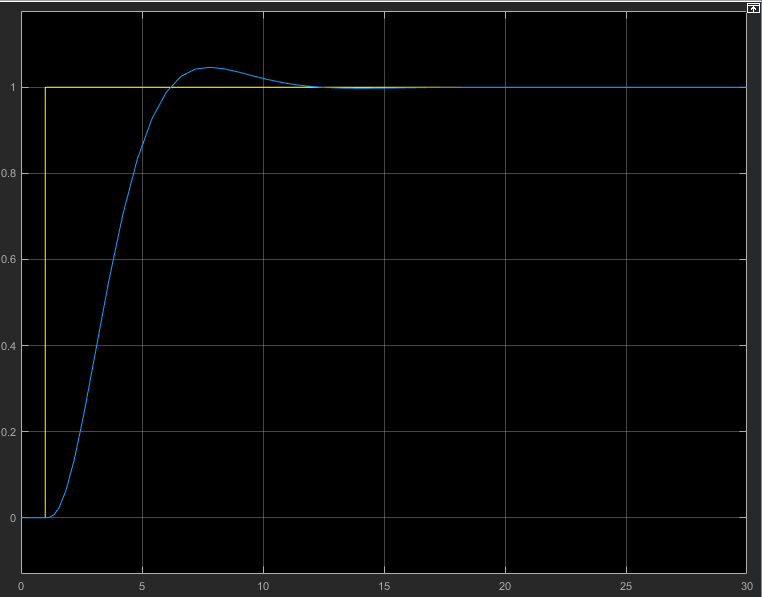
\includegraphics[width=.9\linewidth]{CMVK.png}
		\captionof{figure}{Răspunsul sistemului la intrare treaptă unitară}
		\label{fig:test1}
	\end{minipage}%
	\begin{minipage}{.6\textwidth}
		\centering
		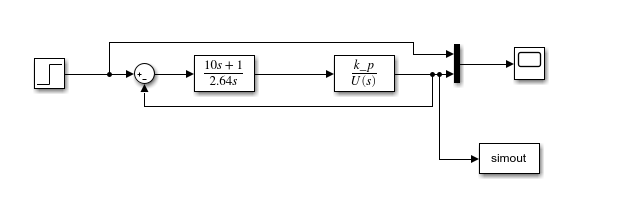
\includegraphics[width=.9\linewidth]{sim_cmvk.png}
		\captionof{figure}{Modelarea procesului în Simulink}
		\label{fig:test2}
	\end{minipage}
\end{figure}
\begin{center}
	\captionof{table}{Performanțe}
	\begin{tabular}{|c|c|c|c|c|c|c|}
		\hline
		&$e_{st}$&$M_v$&$t_s$&$K_r$&$T_i$\\
		\hline
		Impus&0&1&3&-&-\\
		\hline
		Obtinut&0&4.56&9.04&3.78&10\\
		\hline
	\end{tabular}
\end{center}
Avand in vedere lucrarea experimentala 2 unde s-au observat efectele modificarii parametrilor regulatorului asupra indicatorilor de calitate, s-a incercat atingerea performantelor impuse prin incercari.
Pentru implementarea cu incercari s-a pornit de la urmatoarea forma a regulatorului PID prezenta in lucrarea 6:
\begin{equation} 
G_r(s)=k_r(1+\frac{1}{T_i}+\frac{sT_d}{sT_f+1})
\end{equation}
Folosind modelul simulink din Fig.3.
După ulterioare încercari de a modifica coeficienții regulatorului s-au obținut performanțele din Tab. 3 si Fig.3:
\EqRow
\begin{figure}[H]
	\centering
	\begin{minipage}{.4\textwidth}
		\centering
		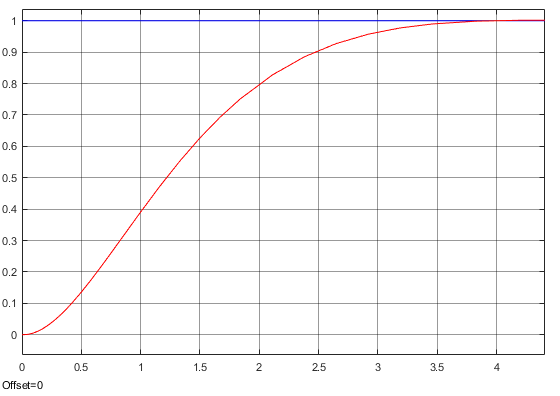
\includegraphics[width=.9\linewidth]{incercari.png}
		\captionof{figure}{Raspunsul celui mai performant sistem din incercari}
		\label{fig:test2}
	\end{minipage}
	\begin{minipage}{.5\textwidth}
		\centering
		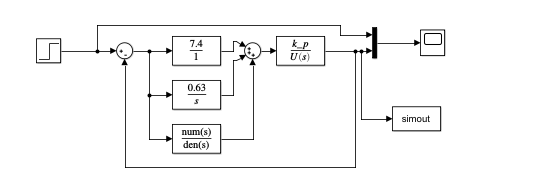
\includegraphics[width=1\linewidth]{sim_incercari.png}
		\captionof{figure}{Model PID folosit pentru incercari}
		\label{fig:test2}
	\end{minipage}
\end{figure}
\begin{center}
	\captionof{table}{Incercari experimentale}
	\begin{tabular}{|c|c|c|c|c|c|c|c|}
		\hline
		&$e_{st}$&$M_v$&$t_s$&$K_r$&$T_i$&$T_d$\\
		\hline
		Impus&0&1&3&-&-&-\\
		\hline
		Obtinut&0&0.06&3.89&7&10&0.8\\
		Obtinut&0&0.19&3.3&7.3&11&0.7\\
		Obtinut&0&0.09&3.2&7.4&11.6&0.67\\
		\hline
	\end{tabular}
\end{center}
\newpage
\subsection{Metode experimentale de proiectare a regulatoarelor PID: metoda Ziegler-Nichols}
Pentru a aplica metoda experimentala este nevoie ca prima oara sa se inregistreze valoarea raspunsului sistemului in bucla deschisa la marimea de intrare treapta unitara.\\
\begin{figure}[H]
	\centering
	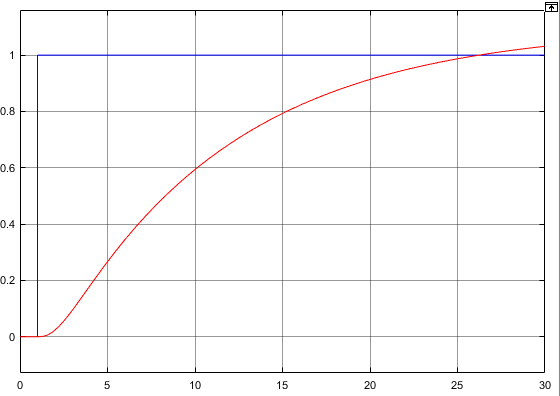
\includegraphics[width=.35\linewidth]{zn_desc.png}
	\captionof{figure}{Raspunsul sistemului in bucla deschisa}
	\label{fig:test2}
\end{figure}
Avand aceste date putem calcula derivata de ordinul I. In continuare se va calcula punctul de maxim al derivatei de ordinul I si se va verifica in datele derivatei de ordinul II daca punctul de maxim indeplineste conditiile de a fi punct de inflexiune.
O data gasit acest punct de inflexiune se va trasa tangenta la graficul raspunsului sistemului prin punctul de inflexiune. Se gasesc punctele de intersectie cu axele $x$ si $y$. \\
\begin{figure}[H]
	\centering
	\begin{minipage}{.5\textwidth}
		\centering
		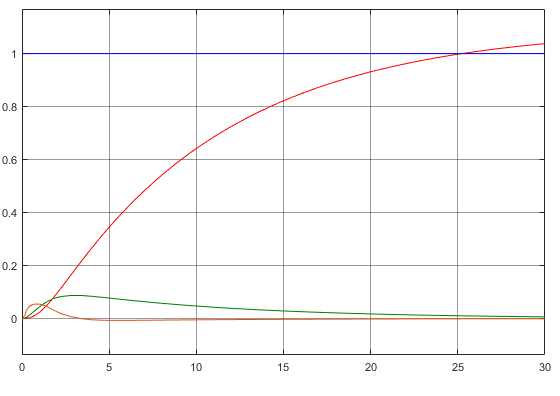
\includegraphics[width=.9\linewidth]{zn_pr.png}
		\captionof{figure}{Răspunsul sistemului si derivatele de ordin I si II}
		\label{fig:test1}
	\end{minipage}%
	\begin{minipage}{.5\textwidth}
		\centering
		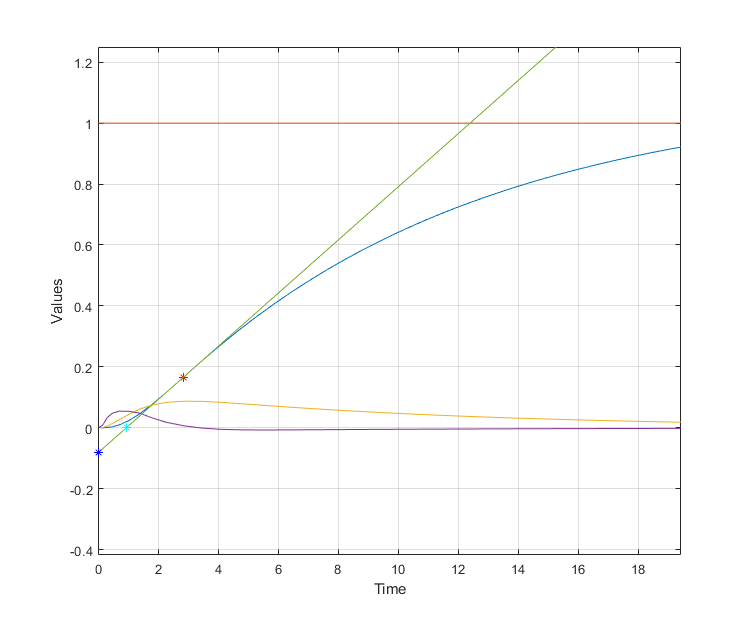
\includegraphics[width=.9\linewidth]{zn_pct.png}
		\captionof{figure}{Puncte necesare pentru proiectare}
		\label{fig:test2}
	\end{minipage}
\end{figure}
Aceste puncte de intersectie semnifica valorile $a$ si $L$ din algoritmul metodei experimentale care se vor folosi pentru a obtine valorile estimate ale coeficientilor regulatorului dupa cum urmeaza: 
\subsection{Proiectarea unui sistem de reglare după stare}
%Random citation \cite{DUMMY:1} embedded in text.
\newpage

\section{Concluzii}

\newpage
\bibliography{bibliografie}
\bibliographystyle{ieeetr}

\end{document}